\documentclass{article}
\usepackage{amsmath}
\usepackage{array}
\usepackage{color}
\usepackage{graphicx}
\usepackage{float} %utiliser H pour forcer � mettre l'image o� on veut
\usepackage{lscape} %utilisation du mode paysage
\usepackage{mathbbol} % permet d'avoir le vrai symbol pour les reels grace a mathbb
\usepackage{enumerate}
\usepackage{marvosym}	
\usepackage{moreverb} % permet d'utiliser verbatimtab : conservation la tabulation 


\setlength {\textwidth}{16cm}
\setlength {\textheight}{21cm} 
\setlength {\oddsidemargin}{0cm}
\setlength{\headsep}{5pt} 

\newcommand\bn{\boldsymbol{\nabla}}
\newcommand\bo{\boldsymbol{\Omega}}
\newcommand\br{\mathbf{r}}
\newcommand\la{\left\langle}
\newcommand\ra{\right\rangle}
\newcommand\bs{\boldsymbol}
\newcommand\red{\textcolor{red}}

\renewcommand{\(}{\left(}
\renewcommand{\)}{\right)}
\renewcommand{\[}{\left[}
\renewcommand{\]}{\right]}

\newtheorem{theorem}{Theorem}[section]

\begin{document}
\title{\textsc{\huge{Simulated annealing }}}
\author{Bruno Turcksin} 
\date{}
\maketitle

\section{Simulated annealing}
We try to solve the well-known problem using the simulated annealing. The advantage of the simulated annealing over the deterministic method is that it can escape a local minima. Unlike the deterministic methods which have to ``go down'' the objective function, the simulated annealing can ``go up''. The disadvantage of the simulated annealing is that the convergence can be very slow.

We try 3 different simulated annealing : the one in scipy, one written by Richard J. Wagner and asamin. 

\section{Equations}
We recall briefly the equations :
\begin{align}
f &= \sum_{(i,j)\in \mathcal{T}}(D_{ij}-\delta_{ij})^2\\
h_1 &= \gamma - \sum_{(i,j)\in \mathcal{D}} \frac{V_{ij}}{V} \nu\(D_{ij}-\delta_{ij}\)\geq 0\\
h_2 &= J \geq 0
\end{align}

\section{Results}
We show the results for the usual 3 test cases with the 3 algorithms.
\subsection{Test 1}
\subsubsection{Scipy}
The minimal value of the function was 0.680299862714. It took 20s to find it. The intensity of the left beam was 0.32550085 and the intensity of the bottom beams was 3.15335189. The dose was :
\begin{table}[H]
\begin{center}
\begin{tabular}{|c|c|c|c|c|}
\hline
0.02068034 & 0.02703252 &  0.01982628 & 0.01119424 &  0.00551321\\
\hline
0.09836511 &  0.09121046 & 0.05862698 & 0.02898301 &  0.01187892\\
\hline
0.80277426  & 0.38263719 & 0.17519708 & 0.06985608 &  0.02607601\\
\hline
0.1 &  0.09763381 & 0.09091342 &  0.03540637 & 0.01351381\\
\hline
0.02224595 &  0.03595995 & 0.1 &  0.02012167 & 0.00707882 \\
\hline
\end{tabular}
\end{center}
\end{table}
\subsubsection{Wagner}
The minimal value of the function was 0.68057082928. It took 42s to find it. The intensity of the left beam was 0.32174478 and the intensity of the bottom beam was 3.15384659. The dose was :
\begin{table}[H]
\begin{center}
\begin{tabular}{|c|c|c|c|c|}
\hline
0.00705558 &  0.01348464 &  0.02605919 &  0.01186862 &  0.00550804\\
\hline
 0.02000732 &   0.03530507 & 0.0698043 & 0.02895584 &  0.01118291\\
\hline
 0.09904863 & 0.09047219 & 0.17503283 & 0.05855832 &  0.01980007\\
\hline
 0.03584808 &  0.09754228 &  0.38263447 &  0.09119305 & 0.02702367\\
\hline
 0.02222509 &  0.0999844 & 0.80287929 &  0.09836838  & 0.02067755 \\
\hline
\end{tabular}
\end{center}
\end{table}
\subsubsection{Asamin}
\subsection{Test 2}
\subsubsection{Scipy}
The minimal value of the function was 1.04934932601. It took 20s to find it. The intensity of the left beam was  0.32435294 and the intensity of the bottom beams was   3.20644137. The dose was :
\begin{table}[H]
\begin{center}
\begin{tabular}{|c|c|c|c|c|}
\hline
 0.00715561 & 0.01368685 &  0.02647862 &  0.01205773 &  0.00559552\\
\hline
 0.02025587 & 0.03581645 & 0.07092294 &  0.02941575  &  0.01135992\\
\hline
 0.1  & 0.09165105 &  0.17781288 & 0.05947846 &  0.02010902\\
\hline
0.0363608 &  0.09909154 & 0.38896999 &  0.09269085 & 0.02746485\\
\hline
 0.0225781 &  0.10162912 & 0.81625328 &   0.1  & 0.02101801 \\
\hline
\end{tabular}
\end{center}
\end{table}
\subsubsection{Wagner}
The minimal value of the function was 1.04966579744. It took 41s to find it. The intensity of the left beam was 0.32258544  and the intensity of the bottom beam was 3.20585418. The dose was :
\begin{table}[H]
\begin{center}
\begin{tabular}{|c|c|c|c|c|}
\hline
 0.00714338 &  0.01367031 &  0.02646439 &  0.01205007 & 0.00559179\\
\hline
  0.02019944 &  0.03576195 & 0.0708818 & 0.02939613  &  0.01135197 \\
\hline
 0.09954781 &  0.0914299 & 0.1776943 & 0.05943264 &  0.02009218\\
\hline
 0.03630142 &  0.09902546 &   0.38887061 &  0.09265964 & 0.02745395\\
\hline
  0.02256304 & 0.10159647 &  0.81609441 &   0.09997623  & 0.02101145 \\
\hline
\end{tabular}
\end{center}
\end{table}
\subsubsection{Asamin}
\subsection{20 beams}
\subsubsection{Scipy}
If we run the code several times, we don't get the same answer. Here we show the best answer :
%\begin{itemize}
%\item The minimal value of the function was  0.469364651845. It took 76s to find it. The intensity of the beams were :
%\begin{table}[H]
%\begin{center}
%\begin{tabular}{|c|c|c|c|c|c|}
%\hline
%Beams & \multicolumn{5}{c|}{Intensity}\\
%\hline
%Left & 4.14750375e-02 & 2.45988947e-03 &  9.97242668e-02 & 7.97332691e-04 & 6.17462049e-03\\
%Right & 6.40920231e-04 & 6.39293084e-04 & 1.81464770e+00 & 5.22410012e-02 & 4.74888980e-01 \\
%Bottom & 3.16624480e-04 &  2.60832145e-03 & 2.13549984e+00 & 2.75848897e-03 &  1.52617788e-02\\
%Top & 7.15346918e-04 & 6.49397239e-04 &  1.67475272e+00 &1.25826366e+00& 3.41721201e-01\\
%\hline
%\end{tabular}
%\end{center}
%\end{table}
%\begin{figure}[H]
%\centering
%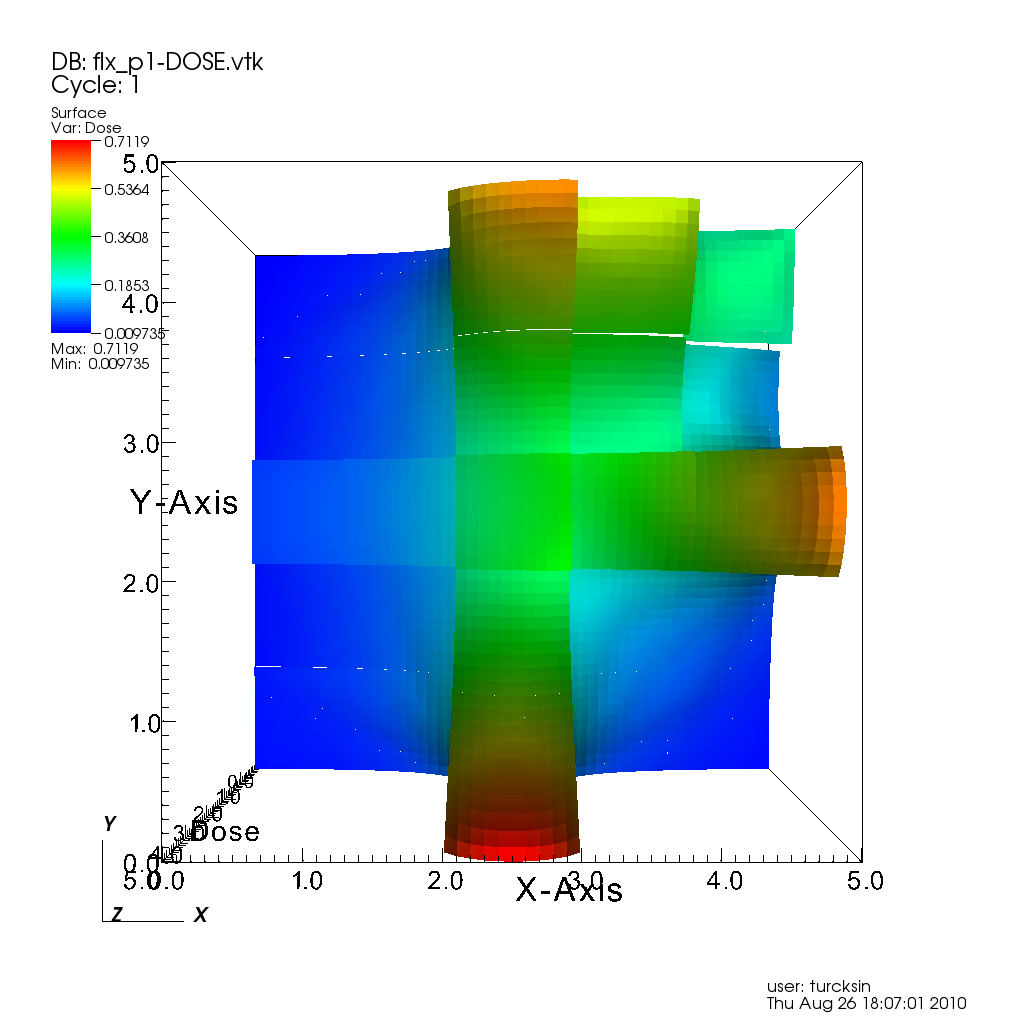
\includegraphics[width=0.5\linewidth]{20b_scipy}
%\end{figure}
%\item 
The minimal value of the function was 0.375748180308. It took 80s to find it. The intensity of the beams were :
\begin{table}[H]
\begin{center}
\begin{tabular}{|c|c|c|c|c|c|}
\hline
Beams & \multicolumn{5}{c|}{Intensity}\\
\hline
Left & 2.38253621e-02 & 5.33177946e-04 &   1.49055863e-01 &  2.85430982e-02 & 2.04711667e-03\\
Right &  2.83815662e-01 & 7.36487483e-01 & 5.99601642e+00 & 7.41488566e-01 & 2.49000466e-03 \\
Bottom & 9.81766473e-03  & 1.11312735e-03 &  4.72456523e-01 &  3.51402213e-01 &  2.14049829e+00\\
Top & 4.72643123e-02 & 7.44557177e-04 &  1.67308985e-01 &3.45692138e-02&  5.59475951e-02\\
\hline
\end{tabular}
\end{center}
\end{table}
Dose :
\begin{table}[H]
\begin{center}
\begin{tabular}{|c|c|c|c|c|}
\hline
  0.02912935 &  0.03882852 &   0.09998867 &  0.09840914 &  0.09416373\\
\hline
   0.04993294 &  0.09038965  & 0.18630418 &  0.30313842  & 0.42985556 \\
\hline
  0.09977892 &  0.17369011 &  0.38701698 & 0.82742674 &  1.68067842\\
\hline
 0.04345325 &  0.09981673 &  0.23552605 &  0.38537144 & 0.64156088\\
\hline
   0.02888053  & 0.05685939 &   0.20673887  &  0.27150366   &  0.67631671 \\
\hline
\end{tabular}
\end{center}
\end{table}
\begin{figure}[H]
\centering
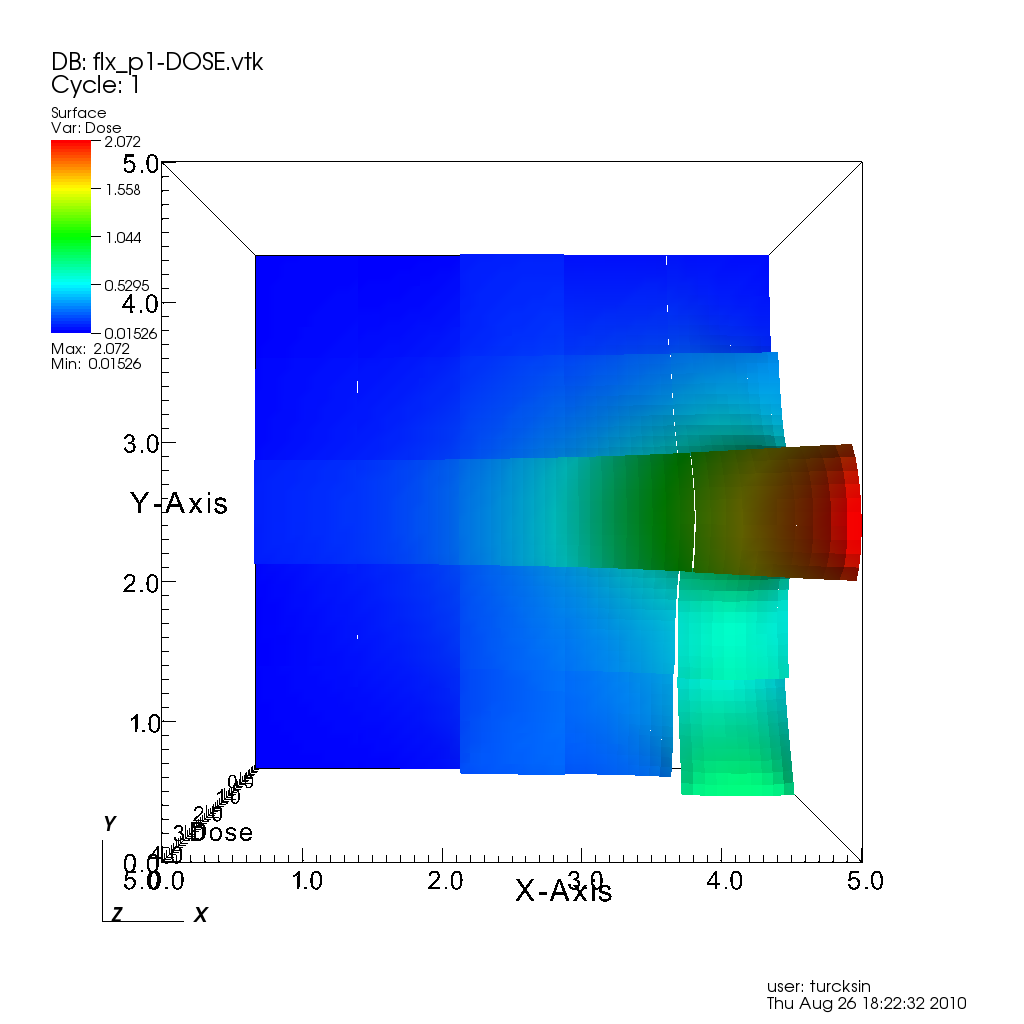
\includegraphics[width=0.5\linewidth]{20b_scipy2}
\end{figure}
%\end{itemize}
\subsubsection{Wagner}
If we run the code several times, we don't get the same answer. Here we show the best answer :
The minimal value of the function was 0.558003521489. It took 179s to find it. The intensity of the beams were :
\begin{table}[H]
\begin{center}
\begin{tabular}{|c|c|c|c|c|c|}
\hline
Beams & \multicolumn{5}{c|}{Intensity}\\
\hline
Left &  2.07006618 &  0.69620052 &   0.93980463 &  0.00516926 &  0.13054651\\
Right &   0.01494169 & 0.07608557 & 0.04902098 & 0.0095044 &  0.27217087 \\
Bottom & 0.30925232  & 0.55016687 &  3.14891157 &   0.04036021 &  0.17741137\\
Top & 0.17376821 &  0.02502432  &  0.07538271 &0.00738365& 0.05280104\\
\hline
\end{tabular}
\end{center}
\end{table}
Dose :
\begin{table}[H]
\begin{center}
\begin{tabular}{|c|c|c|c|c|}
\hline
  0.09583996 &  0.06168959 & 0.07635935 & 0.05807728 & 0.09215599\\
\hline
 0.08445043 &  0.09555408   & 0.11528065 & 0.06045733   & 0.04014426 \\
\hline
0.32410605 & 0.24280889 &  0.25300367 & 0.10631148 & 0.06072916\\
\hline
 0.34674847 &  0.33189023 & 0.48696132 &  0.15413559  &  0.08665099\\
\hline
 0.65417669  &  0.50750915 &  0.93413603  &  0.16653313  &  0.09029707 \\
\hline
\end{tabular}
\end{center}
\end{table}
\begin{figure}[H]
\centering
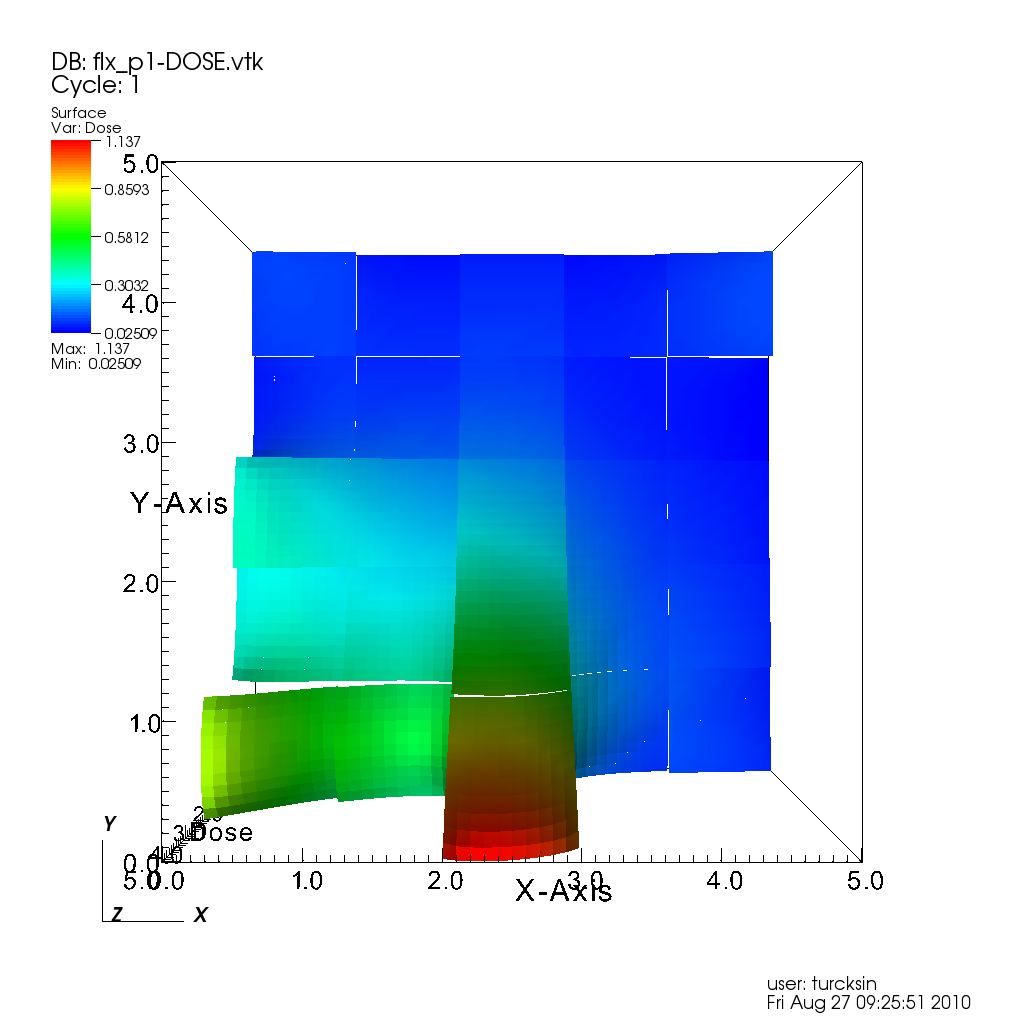
\includegraphics[width=0.5\linewidth]{20b_wagner}
\end{figure}
\subsubsection{Asamin}

\subsection{Cross target}
\subsubsection{Scipy}
If we run the code several times, we don't get the same answer. Here we show the best answer :
The minimal value of the function was 1.5594166666. It took 76s to find it. The intensity of the beams were :
\begin{table}[H]
\begin{center}
\begin{tabular}{|c|c|c|c|c|c|}
\hline
Beams & \multicolumn{5}{c|}{Intensity}\\
\hline
Left &  6.81691519e-01 &  2.14063550e+00 &    2.64252320e+00 &  2.44474154e-01 &   1.79031322e-02 \\
Right &   2.59267734e-03 &  1.00010683e-03 & 1.39903176e-02 & 1.33872040e-03 &  8.46819235e-03 \\
Bottom & 3.36637047e+00  &  2.00402424e+00 &  1.80149275e-03 &  4.97740428e-07 &   1.22594284e-03 \\
Top & 1.48769548e-01 &  4.42905814e-03  & 7.41076506e-04 & 7.68347628e-04 & 4.48483494e-03\\
\hline
\end{tabular}
\end{center}
\end{table}
Dose :
\begin{table}[H]
\begin{center}
\begin{tabular}{|c|c|c|c|c|}
\hline
  0.09743655 &  0.06792597 & 0.0386917  & 0.02143917 &  0.01238235\\
\hline
 0.25074162 &  0.19456834 & 0.09999068 & 0.04896475   & 0.02168415 \\
\hline
0.93880273 & 0.54216739 &  0.22962316  & 0.09851655 &  0.04171066\\
\hline
 1.08016215 &  0.67772646 &  0.24726852 &  0.09989779  & 0.03792243\\
\hline
 1.14299766  & 0.76339284  & 0.16234091  &  0.05692628 &  0.02180886 \\
\hline
\end{tabular}
\end{center}
\end{table}
\begin{figure}[H]
\centering
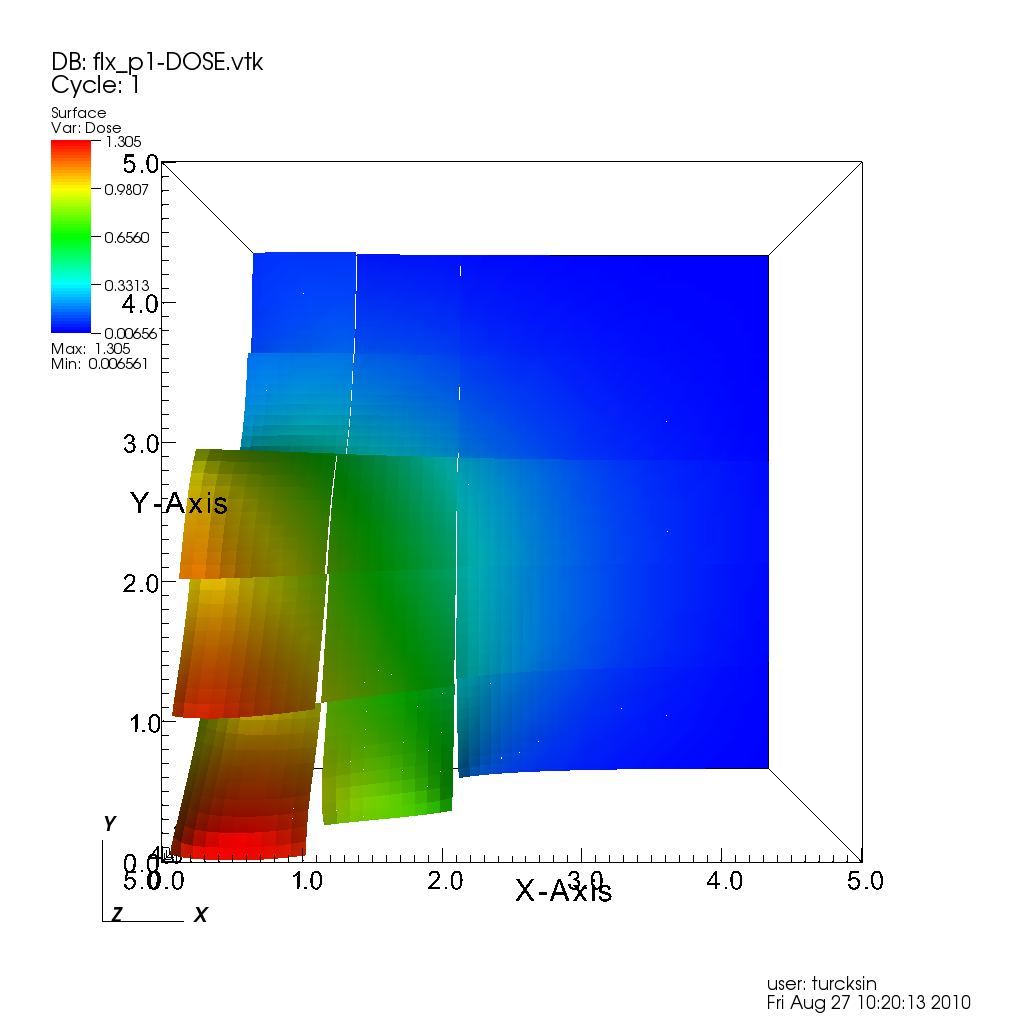
\includegraphics[width=0.5\linewidth]{cross_scipy}
\end{figure}

\end{document}
